\section{Every model at a glance}
\label{sec:glance}

Each model's exact definition, its fitted parameters and what it relies on are in Appendix~\ref{app:models}; this
section summarizes them. Every model is shown at the trace-feature set its A+B cross-validation chose, per target.

\begin{figure}[h]
\centering
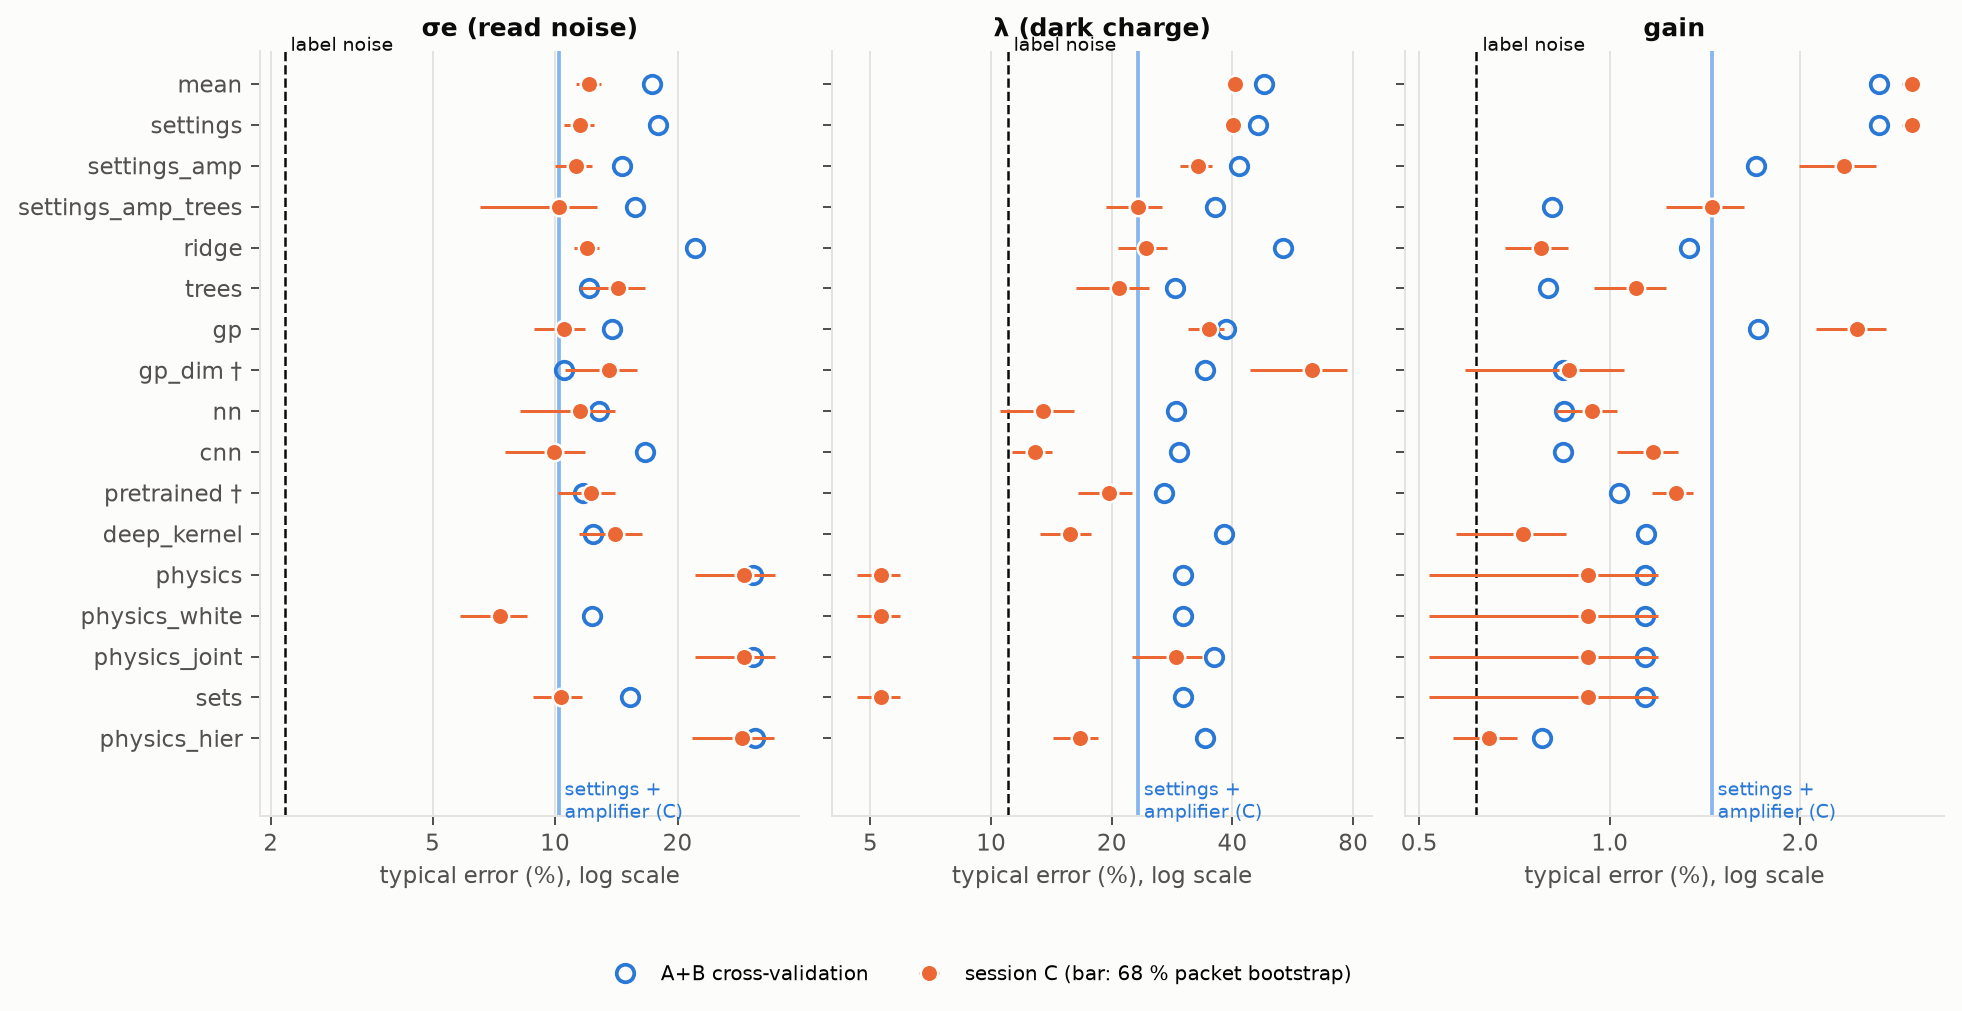
\includegraphics[width=\textwidth]{figures/fig7_all_models.png}
\caption{Every model's error: A+B cross-validation (open) and session C (filled, with the 68\,\% packet-bootstrap
interval), log scale. Vertical lines: settings + amplifier (trees) on session C, and the label noise. $\dagger$: the
frozen choice. The physics models share their $\lambda$ and gain parts.}
\label{fig:all}
\end{figure}

\begin{table}[h]
\centering\scriptsize\renewcommand{\arraystretch}{0.92}
\caption{Every model at the feature set chosen on A+B: errors (\%) and the paired session C difference from settings
+ amplifier (trees), in percentage points with its 95\,\% packet-bootstrap interval (bold: excludes zero), and the
fraction of resamples in which the model is better. $\dagger$: frozen choice.}
\label{tab:all}
\begin{tabular}{llrrrl}
\toprule
model & set (chosen on A+B) & A+B CV & session C & C $-$ settings + amp. [95\,\%] & P(better) \\
\midrule
\multicolumn{6}{l}{\textbf{$\sigma_e$} \quad error in \%; reference: settings + amplifier (trees)} \\
\midrule
\texttt{mean} & none & 17.4 & 12.1 & +1.9 [-2.9, +6.8] & 0.20 \\
\texttt{settings} & none & 17.9 & 11.5 & +1.3 [-3.2, +6.1] & 0.26 \\
\texttt{settings\_amp} & none & 14.6 & 11.2 & +1.0 [-3.6, +6.0] & 0.30 \\
\texttt{settings\_amp\_trees} & none & 15.7 & 10.2 & reference &  \\
\texttt{ridge} & none & 22.0 & 12.0 & +1.8 [-3.4, +6.7] & 0.23 \\
\texttt{trees} & P+A1 & 12.1 & 14.3 & \textbf{+4.1 [+0.6, +9.3]} & 0.01 \\
\texttt{gp} & P+A & 13.8 & 10.5 & +0.3 [-4.1, +5.3] & 0.41 \\
\texttt{gp\_dim}$^{\dagger}$ & P+A1 & 10.5 & 13.5 & +3.3 [-2.9, +10.4] & 0.16 \\
\texttt{nn} & all & 12.8 & 11.5 & +1.3 [-4.7, +8.3] & 0.34 \\
\texttt{cnn} & P+A+B & 16.6 & 10.0 & -0.2 [-3.5, +4.4] & 0.55 \\
\texttt{pretrained} & P+A+B & 11.7 & 12.2 & +2.0 [-2.0, +7.3] & 0.17 \\
\texttt{deep\_kernel} & P+A & 12.4 & 14.1 & +3.9 [-4.3, +11.2] & 0.14 \\
\texttt{physics} & P+A+B & 30.6 & 29.1 & \textbf{+18.9 [+9.2, +30.2]} & 0.00 \\
\texttt{physics\_white} & P+A & 12.3 & 7.3 & -2.9 [-9.3, +3.1] & 0.74 \\
\texttt{physics\_joint} & P+A+B & 30.6 & 29.1 & \textbf{+18.9 [+9.2, +30.2]} & 0.00 \\
\texttt{sets} & P+A1 & 15.3 & 10.3 & +0.1 [-6.9, +6.2] & 0.43 \\
\texttt{physics\_hier} & P+A & 31.0 & 28.8 & \textbf{+18.6 [+7.7, +29.6]} & 0.00 \\
\midrule
\multicolumn{6}{l}{\textbf{$\lambda$} \quad error in \%; reference: settings + amplifier (trees)} \\
\midrule
\texttt{mean} & none & 47.8 & 40.5 & \textbf{+17.3 [+9.4, +25.7]} & 0.00 \\
\texttt{settings} & none & 46.4 & 40.2 & \textbf{+17.0 [+9.0, +25.5]} & 0.00 \\
\texttt{settings\_amp} & none & 41.6 & 32.8 & +9.5 [-0.4, +19.5] & 0.03 \\
\texttt{settings\_amp\_trees} & none & 36.1 & 23.2 & reference &  \\
\texttt{ridge} & P & 53.5 & 24.3 & +1.1 [-10.9, +12.9] & 0.42 \\
\texttt{trees} & all & 28.8 & 20.9 & -2.3 [-16.7, +10.8] & 0.63 \\
\texttt{gp} & P+A1 & 38.6 & 34.9 & \textbf{+11.7 [+1.0, +22.6]} & 0.01 \\
\texttt{gp\_dim} & all & 34.1 & 63.1 & +39.9 [-2.5, +70.7] & 0.04 \\
\texttt{nn} & all & 28.9 & 13.5 & -9.7 [-19.8, +0.1] & 0.97 \\
\texttt{cnn} & all & 29.4 & 12.9 & \textbf{-10.3 [-18.9, -1.6]} & 0.99 \\
\texttt{pretrained}$^{\dagger}$ & all & 27.0 & 19.7 & -3.6 [-14.4, +7.4] & 0.74 \\
\texttt{deep\_kernel} & all & 38.1 & 15.7 & -7.5 [-17.1, +2.3] & 0.93 \\
\texttt{physics} & all & 30.1 & 5.3 & \textbf{-17.9 [-25.8, -10.1]} & 1.00 \\
\texttt{physics\_white} & all & 30.1 & 5.3 & \textbf{-17.9 [-25.8, -10.1]} & 1.00 \\
\texttt{physics\_joint} & all & 35.9 & 28.9 & +5.7 [-8.6, +19.4] & 0.25 \\
\texttt{sets} & all & 30.1 & 5.3 & \textbf{-17.9 [-25.8, -10.1]} & 1.00 \\
\texttt{physics\_hier} & P & 34.1 & 16.6 & -6.6 [-14.8, +1.1] & 0.96 \\
\midrule
\multicolumn{6}{l}{\textbf{gain} \quad error in \%; reference: settings + amplifier (trees)} \\
\midrule
\texttt{mean} & none & 2.7 & 3.0 & \textbf{+1.6 [+1.3, +1.9]} & 0.00 \\
\texttt{settings} & none & 2.7 & 3.0 & \textbf{+1.6 [+1.3, +1.9]} & 0.00 \\
\texttt{settings\_amp} & none & 1.7 & 2.3 & \textbf{+0.9 [+0.5, +1.3]} & 0.00 \\
\texttt{settings\_amp\_trees} & none & 0.8 & 1.4 & reference &  \\
\texttt{ridge} & P+A1 & 1.3 & 0.8 & \textbf{-0.7 [-1.1, -0.1]} & 0.99 \\
\texttt{trees} & P+A+B & 0.8 & 1.1 & \textbf{-0.4 [-0.6, -0.1]} & 0.99 \\
\texttt{gp} & P & 1.7 & 2.5 & \textbf{+1.0 [+0.5, +1.4]} & 0.00 \\
\texttt{gp\_dim}$^{\dagger}$ & P & 0.8 & 0.9 & -0.6 [-1.2, +0.1] & 0.95 \\
\texttt{nn} & P+A+B & 0.8 & 0.9 & -0.5 [-1.0, +0.0] & 0.97 \\
\texttt{cnn} & P+A+B & 0.8 & 1.2 & -0.3 [-0.7, +0.3] & 0.84 \\
\texttt{pretrained} & P+A & 1.0 & 1.3 & -0.2 [-0.5, +0.3] & 0.78 \\
\texttt{deep\_kernel} & P+A1 & 1.1 & 0.7 & \textbf{-0.7 [-1.3, -0.1]} & 0.99 \\
\texttt{physics} & P & 1.1 & 0.9 & -0.5 [-1.3, +0.3] & 0.88 \\
\texttt{physics\_white} & P & 1.1 & 0.9 & -0.5 [-1.3, +0.3] & 0.88 \\
\texttt{physics\_joint} & P & 1.1 & 0.9 & -0.5 [-1.3, +0.3] & 0.88 \\
\texttt{sets} & P & 1.1 & 0.9 & -0.5 [-1.3, +0.3] & 0.88 \\
\texttt{physics\_hier} & P+A1 & 0.8 & 0.6 & \textbf{-0.8 [-1.1, -0.5]} & 1.00 \\
\bottomrule
\end{tabular}

\end{table}

\begin{figure}[h]
\centering
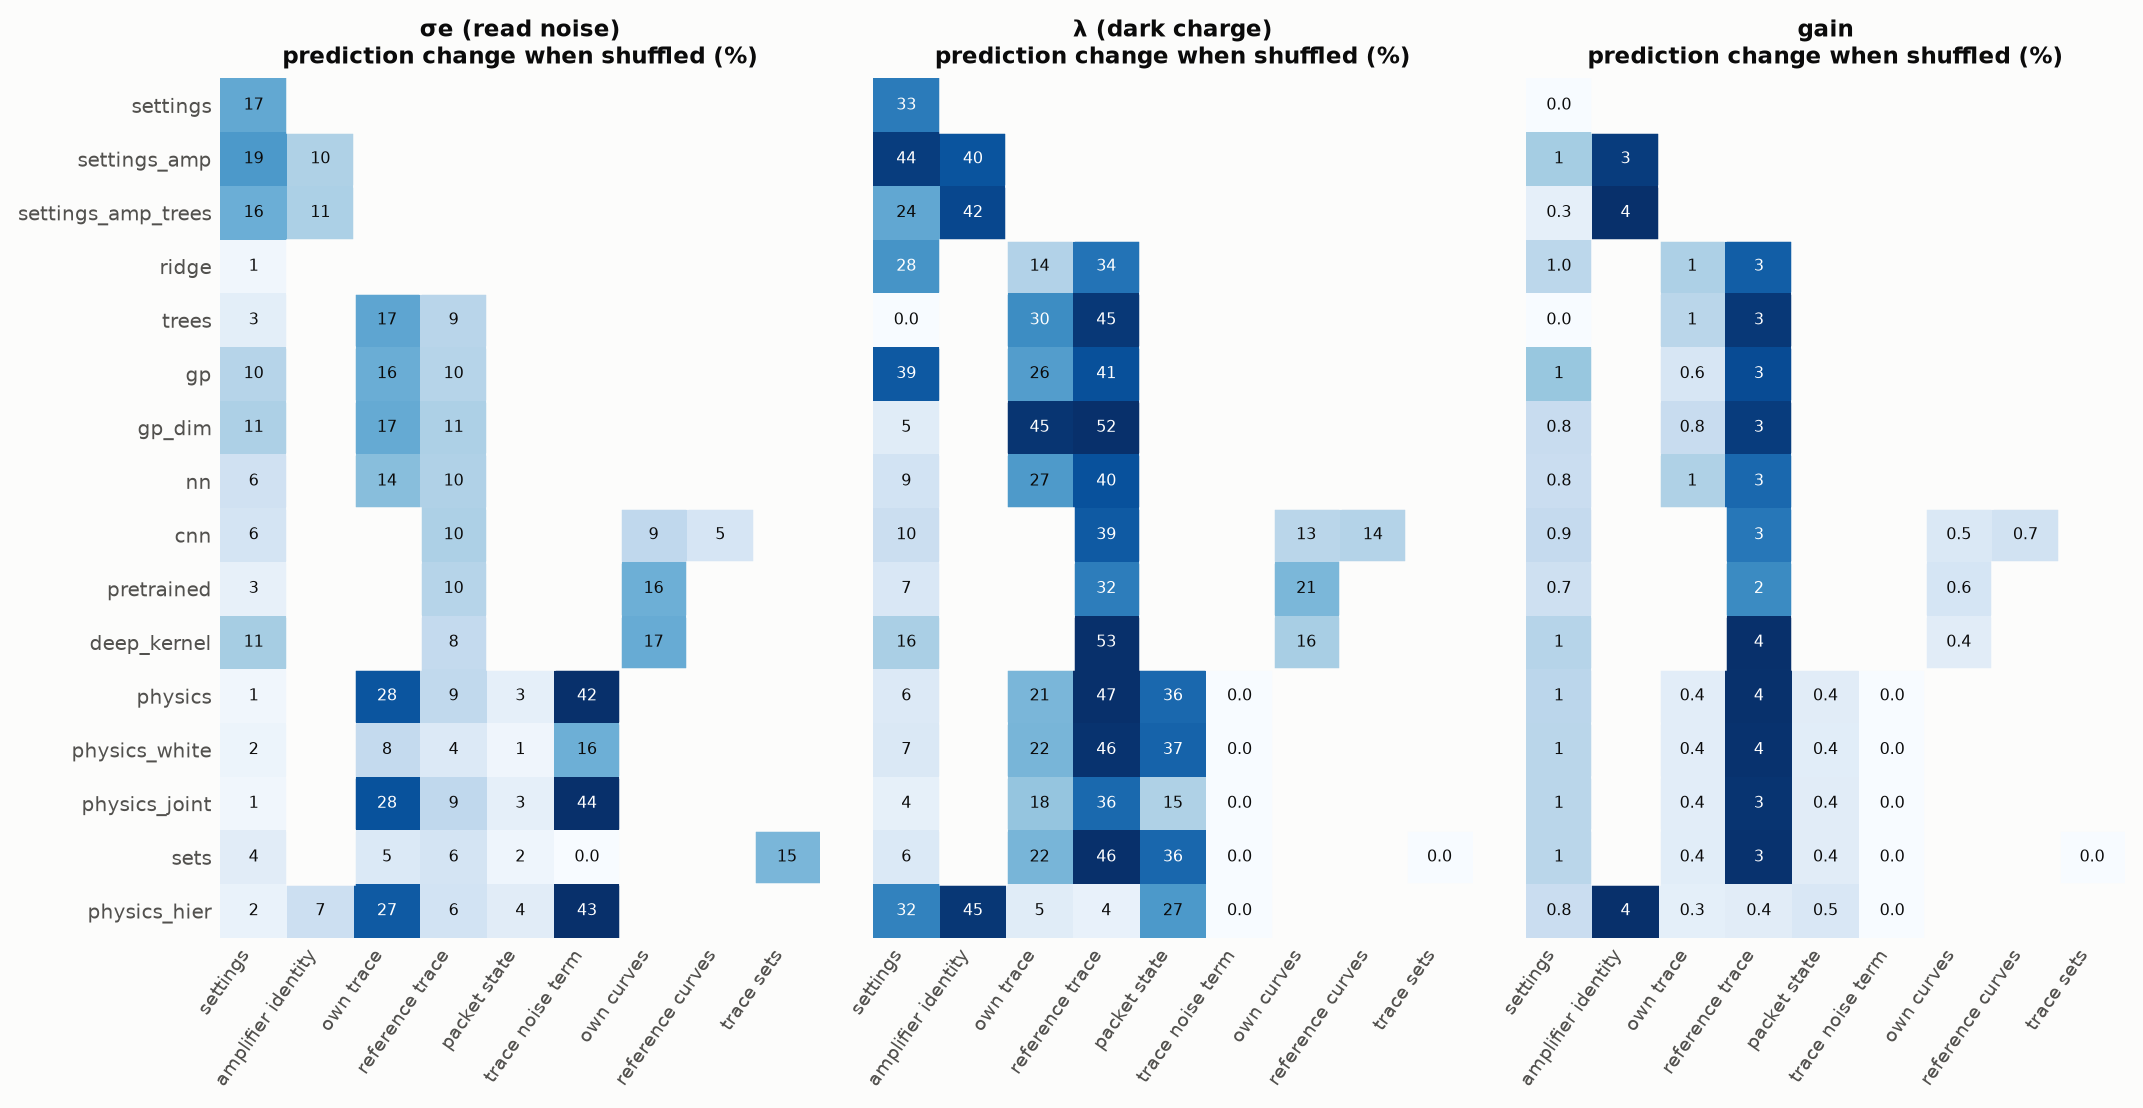
\includegraphics[width=\textwidth]{figures/fig8_reliance.png}
\caption{What every model's predictions move with: the RMS change of the prediction (\% of the target) when one group
of inputs is shuffled across all rows (A+B and C), the model fitted once on A+B. Blank: the model does not see that
group. The trace noise term is used only for $\sigma_e$ by construction.}
\label{fig:reliance}
\end{figure}

\paragraph{What the models rely on} (Fig.~\ref{fig:reliance}; per model, Appendix~\ref{app:models}).
\begin{itemize}
\item \textbf{The gain comes from recognising the amplifier.} Every trace model's gain rests on the reference trace's
  noise features (jump-robust CDS $\sigma$, white noise per skip, null-CDS noise). Shuffled across all rows they move
  the gain by about 3.5\,\%; shuffled only among rows of the same amplifier, by about 0.5\,\%. So the traces tell the
  models \emph{which amplifier} this is, and the gain follows. The settings move it by about 1\,\% (VDD, VR, VDRAIN). The
  gain varies little within an amplifier (repeat scatter 0.6\,\%), so this is most of what there is to learn.
\item \textbf{$\lambda$: the amplifier, the own trace, and the CCD's state.} In the physics family's $\lambda$ GP (the
  best $\lambda$ model, 5.3\,\%) the reference trace moves $\lambda$ by 46\,\% but by only 6\,\% within an amplifier: it
  identifies the amplifier, and shuffling it costs 46 points on C. The own trace moves it by 22\,\% also within an
  amplifier and costs 18 points on C: it carries information about this packet beyond the amplifier. The packet state
  moves the predictions by 37\,\% but costs nothing on C: what it learned about the CCD's drift in A+B does not carry
  over to session C. The settings move $\lambda$ by 6\,\%. The SAAS prior keeps few inputs, and a single one (the
  reference trace's edge jitter) moves $\lambda$ by 58\,\%: a fragile point for a new night.
\item \textbf{$\sigma_e$: the measured noise versus proxies.} \texttt{physics\_white}'s $\sigma_e$ rests on the trace's
  white noise (moves 16\,\%, costs 5 points on C when shuffled); its correction uses own-trace features
  (permutation entropy, line frequency, row-start ratio, transient time constant). The flexible models (gp\_dim,
  trees, nn) rely instead on own-trace timing proxies (row-start recovery time, CDS ringing in skips 1--4) and the
  settings, and never on a noise measurement directly; they fit the A+B timing packets and fail on C. \texttt{physics}
  leans on the Allan floor (42\,\%), the unstable term that gives it 29\,\%.
\item \textbf{The references.} The settings-only GP moves $\lambda$ with delayInt and the RG low levels and does not
  move the gain at all. settings + amplifier (trees) uses only five inputs: delayInt and the four amplifier columns.
  With at least 10 rows per leaf, a knob changed in one or two A+B packets can never be split on. The labelled
  \texttt{physics\_hier} predicts $\lambda$ from the amplifier identity (45\,\%) and the settings (32\,\%) and is worse on C
  (16.6\,\%) than the label-free physics model, which identifies the amplifier from its traces and also reads its state.
\end{itemize}

\begin{figure}[h]
\centering
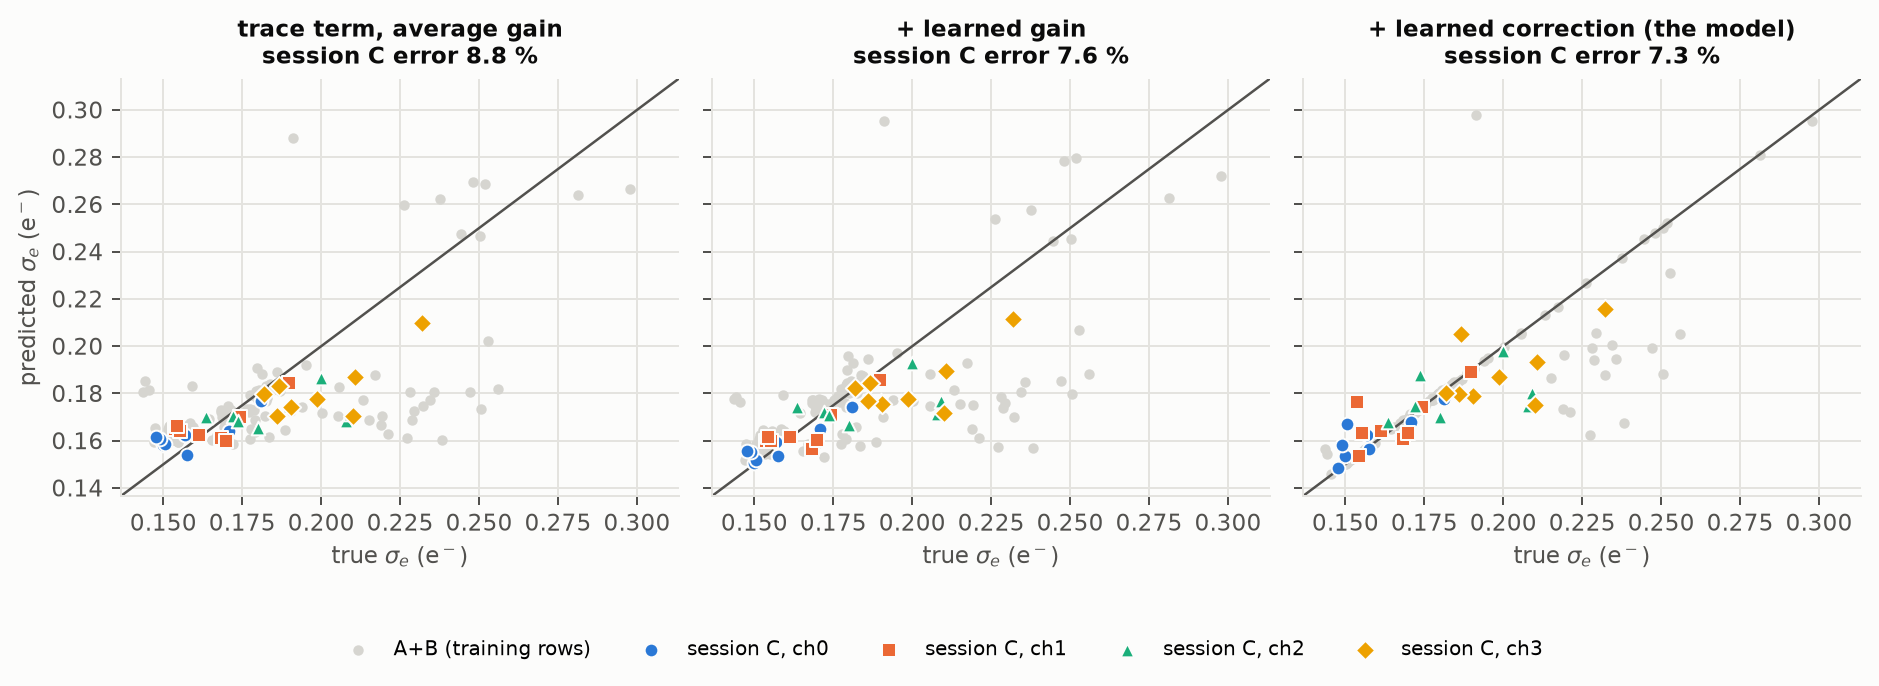
\includegraphics[width=\textwidth]{figures/fig9_physics_terms.png}
\caption{The physics-structured $\sigma_e$ (physics\_white [P+A]) built up term by term: the trace's white noise
$/\sqrt N$ divided by the average gain, then by the learned gain, then with the learned correction. Most of the
session C accuracy comes from the measured noise. In A+B (grey; training rows, so the right panel is in-sample) the
trace term alone misses the timing packets; the correction pulls them in.}
\label{fig:terms}
\end{figure}

\paragraph{Caveats.} Shuffling measures what a fitted model uses, not what is causally true; correlated inputs share
credit (hence the group shuffles). The network models were refitted for this analysis, and with their random starts
their session C errors differ from the scored run by up to 2 points (the tables report the scored run).
